\subsection{圣诞节}

圣诞节又称耶诞节,译名为“基督弥撒”,它源自古罗马人迎接新年的农神节,与基督教本无关系。在基督教盛行罗马帝国后,教廷随波逐流地将这种民俗节日纳入基督教体系,同时以庆祝耶稣的降生。但在圣诞节这天不是耶稣的生辰,因为《圣经》未有记载耶稣具体生于哪天,同样没提到过有此种节日,是基督教吸收了古罗马神话的结果。大部分的天主教教堂都会先在12月24日的平安夜,亦即12月25日凌晨举行子夜弥撒,而一些基督教会则会举行报佳音,然后在12月25日庆祝圣诞节;基督教的另一大分支——东正教的圣诞节庆则在每年的1月7日。圣诞节也是西方世界以及其他很多地区的公共假日,例如:在亚洲的中国香港和澳门地区、马来西亚、新加坡。4世纪初,1月6日是罗马帝国东部各教会纪念耶稣降生和受洗的双重节日、称为“主显节”(Epiphany),亦称“显现节”,即上帝通过耶稣向世人显示自己。当时只有那路拉冷的教会例外,那里只纪念耶稣的诞生而不纪念耶稣的受洗。后历史学家在罗马基督徒习用的日历中发现公元354年12月25日页内记录着:“基督降生在犹大的伯利恒。”经研究,一般认为12月25日伴为圣诞节可能开始于公元336年的罗马教会,约在公元375年传到小亚细亚的安提阿,公元430年传到埃及的亚历山大里亚,那路撒冷的教会接受得最晚,而亚美尼亚的教会则仍然坚持1月6日主显节是耶稣的诞辰。

\begin{itemize}
\item \emph{圣诞卡}

 圣诞卡(圣诞卡片)在美国和欧洲很流行,许多家庭随贺卡带上年度家庭合照或家庭新闻,新闻一般包括家庭成员在过去一年的优点特长等内容。圣诞节以和平与仁爱的方式达成天下一家的理想。寄赠圣诞卡,除表示庆贺圣诞的喜乐外,就是向亲友祝福,以表怀念之情。尤其对在孤寂中的亲友,更是亲切的关怀和安慰。

 \begin{figure}[htb]
    \centering
    
\includegraphics[width=0.6\linewidth]{sdkp}
    \caption{圣诞卡片}
 \end{figure}

\item \emph{圣诞帽}

 是一顶红色帽子,据说晚上戴上睡觉除了睡得安稳和有点暖外,第二天你还会发现在帽子里多了点心爱的人送的礼物。圣诞装饰包括以圣诞装饰和圣诞灯装饰的圣诞树,户内以花环和常绿植物加以装饰,特别的冬青和槲寄生是传统采用的材料。在南北美洲和少数欧洲地区,传统上户外以灯光装饰,包括用灯火装饰的雪橇、雪人和其他圣诞形象。冬青和槲寄生是传统采用的材料。市政当局也会对圣诞装饰加以支持,在街道悬挂圣诞标语或者是在广场放置圣诞树。
 \begin{figure}[htb]
     \centering
     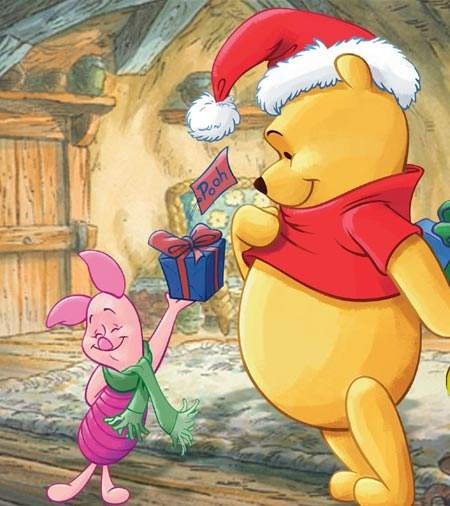
\includegraphics[width=0.3\linewidth]{sdm}
     \caption{圣诞帽}
 \end{figure}

\item \emph{圣诞树}

 圣诞树(Christmas tree)是圣诞节庆祝中最有名的传统之一。通常人们在圣诞前后把一棵常绿植物如松树弄进屋里或者在户外,并用圣诞灯和彩色的装饰物装饰。并把一个天使或星星放在树的顶上。用灯烛和装饰品把枞树或洋松装点起来的常青树,作为圣诞节庆祝活动的一部分。圣诞树起源于德国。很久以前,罗马异教徒就用常青树的树枝装饰房子,寓意度过寒冷冬季之后的生命轮回。到了16世纪,德国人开始把常青树放到家中进行装饰。到了19世纪末,欧洲移民把圣诞树带入了美国殖民地并逐渐流传于世界各地。德国人于每年12月24日,即亚当和夏娃节,在家里布置一株枞树(伊甸园之树),将薄饼干挂在上面,象征圣饼(基督徒赎罪的标记)。近代改用各式小甜饼代替圣饼,还常加上象征基督的蜡烛。此外,室内还设有圣诞塔,是一木质的三角形结构,上有许多小架格放置基督雕像,塔身饰以常青树枝叶、蜡烛和一颗星。到16世纪,圣诞塔和伊甸园树合并为圣诞树。圣诞树到底是什么树呢?其实,只要是松柏类、常绿、树形呈三角形的树都可作为圣诞树。

\item \emph{圣诞橱窗}

 圣诞橱窗也是墨尔本一道靓丽的风景线,每年的圣诞节来临前商店的橱窗设计人员就会动足脑筋,将这个圣诞节的主题发挥得淋漓尽致,而且绝不会和往年的风格重合,这里也是妈妈最愿意带孩子们来的地方。圣诞爷爷醇厚的嗓音讲述着惊心动魄的经历,故事还是那个故事,但声、光、电的组合更生动有趣。排队入场是玛雅橱窗参观中不成文的规定,栏杆外是急匆匆路过的人流,栏杆内有序参观,每个橱窗有数分钟的演绎。
\begin{figure}[htb]
    \centering
    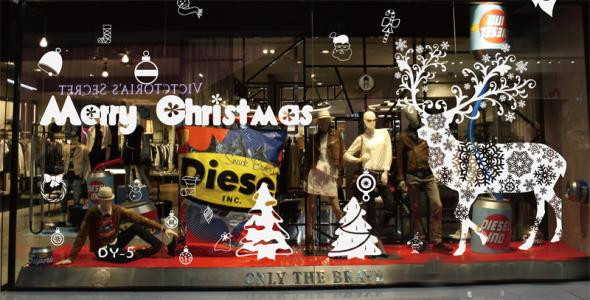
\includegraphics[width=0.4\linewidth]{shendanchuchuan}

    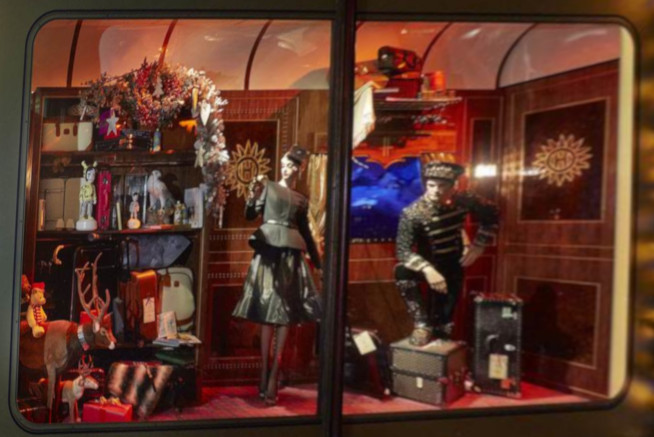
\includegraphics[height=3cm]{shendanchchuan2}    
    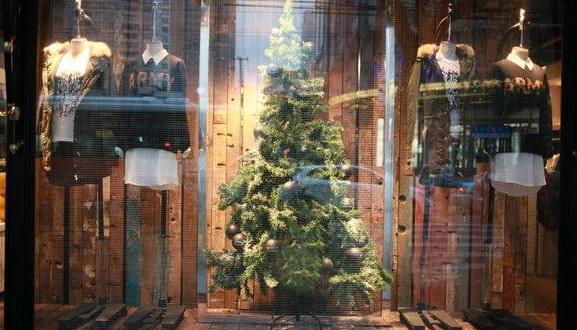
\includegraphics[height=3cm]{shendanchchuan3}
    \caption{圣诞橱窗}
\end{figure}

\end{itemize}

西方国家圣诞节其间挂在家门口用的装饰品,通常用绿色的枝叶或藤条(松毛、松针等)和银色的金属及金色的铃铛配以红色的缎带组成主色调绿、白、黄、红代表欢乐喜庆上面写着MERRY CHRISTMAS或者简写为X'mas,圣诞节环最早出现在芬兰。

\subsubsection{圣诞老人的故事}
一位专门为好孩子在圣诞节前夜送上礼物的神秘人物。传说每到12月24日晚上,有个神秘人会驾乘由12只驯鹿拉的雪橇,挨家挨户地从烟囱进入屋里,然后偷偷把礼物放在好孩子床头的袜子里,或者堆在壁炉旁的圣诞树下。虽然没有人真的见过神秘人的样子,但是人们通常装扮成头戴红色圣诞帽子,大大的白色胡子,一身红色棉衣,脚穿红色靴子的样子,因为总在圣诞节前夜出现派发礼物,所以习惯地称他为"圣诞老人"。1985年和1994年分别有一部同名电影《圣诞老人》公映。圣诞老人源于欧洲的民间传说。通常父母们会对他们的子女解释他们在圣诞节收到的礼物是圣诞老人送的。圣诞老人以一位神秘人物带给小孩子们礼物的概念衍生自圣尼古拉。尼古拉是一位生活在4世纪小亚细亚的好心主教,荷兰人在圣尼古拉斯节(12月6日)便会模仿他送礼物。每年圣诞节,圣诞老人骑在驯鹿上,圣童手持圣诞树降临人间,随着世事变迁,作家和艺术家开始把圣诞老人描述成我们今日熟悉的着红装,留白胡子的形象。同时不同的国度和文化对圣诞老人也有了不同的解释。
\begin{figure}[htb]
    \centering
    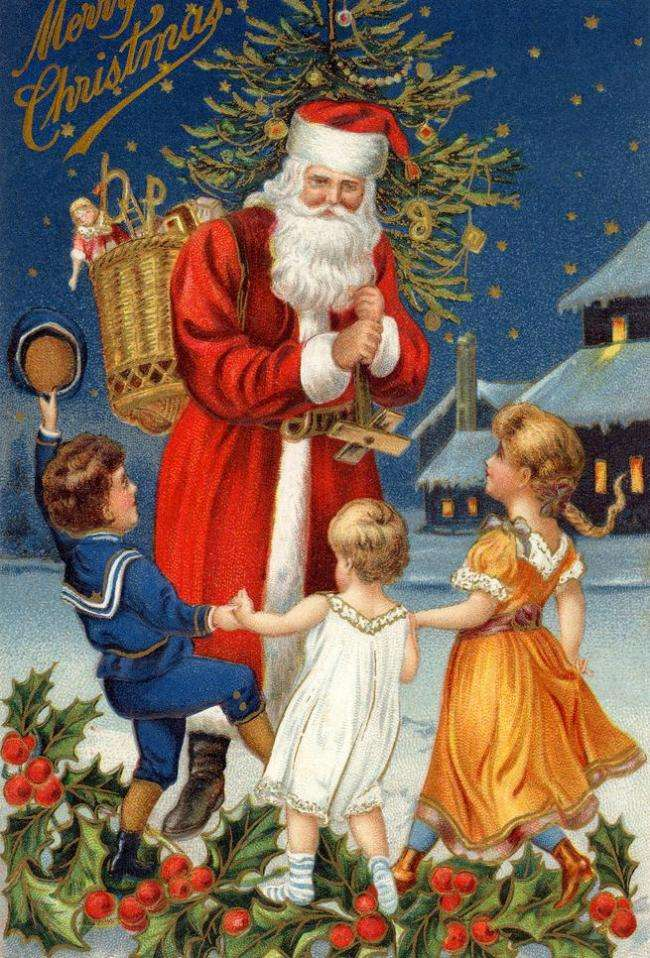
\includegraphics[width=0.3\linewidth]{oldman}
    \caption{圣诞老人}
\end{figure}

在德国,传说他扮成圣童把坚果和苹果放在孩子们鞋里。他乘双轮马车四处漫游,观察人们的行为,尤其是小孩,如果表现好,将会得到苹果、坚果、糖等诸多奖品。坏孩子则得一鞭子。家长们灵机一动纷纷采用此传说来鼓励孩子们听话。大大超过了新年,成为一个全民的节日。圣诞老人已经成为圣诞节最受喜爱的象征和传统。他赶着驯鹿,拉着装满玩具和礼物的雪橇挨家挨户给每个孩子送礼物的快乐老精灵的形象已深深地留在人们的记忆中。每年接近圣诞节,总会有(相信有圣诞老人的)小孩子寄信给圣诞老人,内容如告知其自己希望收的圣诞礼物之类,而在某些国家的邮局,为了免让他们失望,更会有专人回复这些信件。
\subsection{Aschermittwoch}

圣灰星期三,又称圣灰的第四天。圣灰星期三前一天是忏悔星期二。圣灰星期三这个词来自于崇拜前一年烧焦的棕榈树枝骨灰的习俗,并在这一天将这个圣灰称为忠实的十字架。从格雷戈里大帝的教皇以来开始进行四旬斋,四旬斋是为了纪念耶稣在旷野中斋戒和祈祷的40天,是为复活节做准备。